\section{Sprint 6}

\subsection*{Summary}

\begin{table}[H]
	\centering
	\begin{tabular}{ll}
		\toprule
		\multicolumn{2}{c}{\textbf{Sprint 6}}\\
		\midrule
		\textbf{Periode} & 27.04.2015 12:00 Uhr\textendash 11.05.2015 12:00 Uhr\\
		\textbf{Stunden Soll} & \SI{144}{\hour}\\
		\textbf{Stunden Plan} & \SI{151.5}{\hour} \\
		\textbf{Stunden Ist} & \SI{167}{\hour}\\
		\bottomrule
	\end{tabular}
\end{table}

\begin{figure}[H]
	\centering
	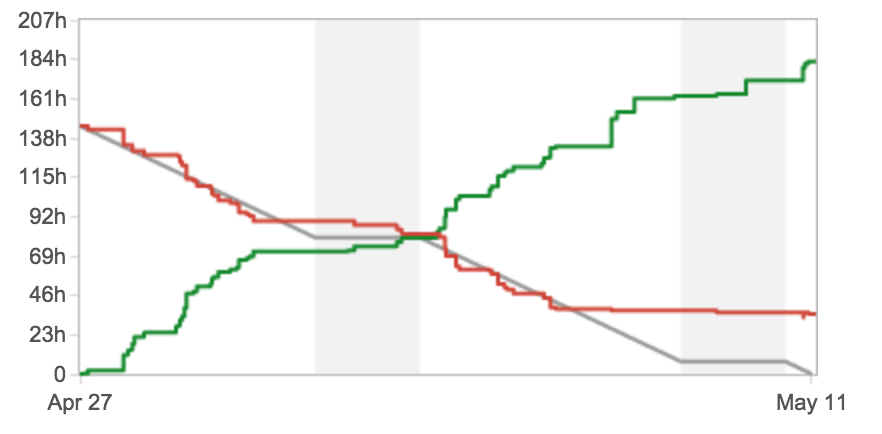
\includegraphics{fig/bd-sprint-6}
	\label{fig:pm:bd-sprint-6}
	\caption*{Burndown Chart Sprint 6}
\end{figure}

\subsection*{Ziele}
Dieser Sprint ist der letzte Feature-Sprint. Insbesondere die Transformationen sollten in ihrer Basisfunktionalität fertig implementiert werden. Zudem sollen die diversen Quellen der \acs{trobdb} sauber mittels \acs{odhql}-Transformationen integriert werden. 

\subsection*{Abgeschlossen}
Folgende High-level (ohne Subtasks) Jira Tasks wurden während Sprint 6 abgeschlossen. 

\begin{table}[H]	
\centering
\begin{tabular}{ll}
	\toprule
	\textbf{JIRA-Key} & \textbf{Summary}\\
	\midrule
DAT-112	Projektmeetings Sprint 6\\
DAT-113	Organisation, Planung \& Kommunikation Sprint 6\\
DAT-114	Übrige Aufwände Sprint 6\\
DAT-115	TROBDB Transformation\\
DAT-116	Template Transformationen\\
DAT-117	Bugfixing\\
DAT-119	OdhQL Benutzerdokumentation\\
	\bottomrule
\end{tabular}	
\end{table}

\subsection*{Probleme}
Die verschiedenen \acs{gdal}-Versionen auf den verschiedenen Systemen (Travis, Heroku, Entwicklung) haben zu unterschiedlichem Verhalten und Fehlern in der Applikation geführt. Neu muss auf allen Systemen die Bibliothek (Version 1.11.1) selbst kompiliert werden (statt via apt-get).